% THIS TEMPLATE IS A WORK IN PROGRESS

\documentclass{article}
\usepackage{graphicx}
\usepackage{hyperref}
\usepackage{fancyhdr}
\usepackage{float}
\usepackage{hyperref}

% FOR CODE
\usepackage{listings}
\usepackage{xcolor}

\definecolor{codegreen}{rgb}{0,0.6,0}
\definecolor{codegray}{rgb}{0.5,0.5,0.5}
\definecolor{codepurple}{rgb}{0.58,0,0.82}
\definecolor{backcolour}{rgb}{0.95,0.95,0.92}

\lstdefinestyle{mystyle}{
    backgroundcolor=\color{backcolour},   
    commentstyle=\color{codegreen},
    keywordstyle=\color{magenta},
    numberstyle=\tiny\color{codegray},
    stringstyle=\color{codepurple},
    basicstyle=\ttfamily\footnotesize,
    breakatwhitespace=false,         
    breaklines=true,                 
    captionpos=b,                    
    keepspaces=true,                 
    numbers=left,                    
    numbersep=5pt,                  
    showspaces=false,                
    showstringspaces=false,
    showtabs=false,                  
    tabsize=2
}

\lstset{style=mystyle}
% 

\fancypagestyle{firstpage}{%
  \lhead{CAP6610 Project Progress Report}
  \rhead{Akash Gajjar}
}

\begin{document}
\thispagestyle{firstpage}

\section{Summary}
For the past few days I have been mainly setting up my local development environment and loading and exploring the data. I have installed \emph{python 3.9.6} on my local machine. I am also using python virtual environment so that I can separate all the python packages for different use cases to different environment and have a \emph{requirements.txt} for the ML virtual environment in case I want to move my work to a separate machine. Apart from that, I have downloaded the MNIST dataset from Kaggle (\url{https://www.kaggle.com/datasets/hojjatk/mnist-dataset}). There are two groups of images, Train and Test. There are total 60,000 samples for training and 10,000 samples for testing. Each image also has it's corresponding label which may not be used in our case. The images have 28x28 dimension and they are in grayscale. In order to load the data using python and explore it, I had to look into \emph{numpy} and \emph{matplotlib} library documentations. I created a class called \emph{MnistDataloader} with help of some of the Jupyter Notebooks available online. I am also learning how to use Jupyter Notebooks and later I plan to use Google Colab for training and testing.

\section{Samples}
Below are some sample images from the DataSet.
\begin{figure}[H]
  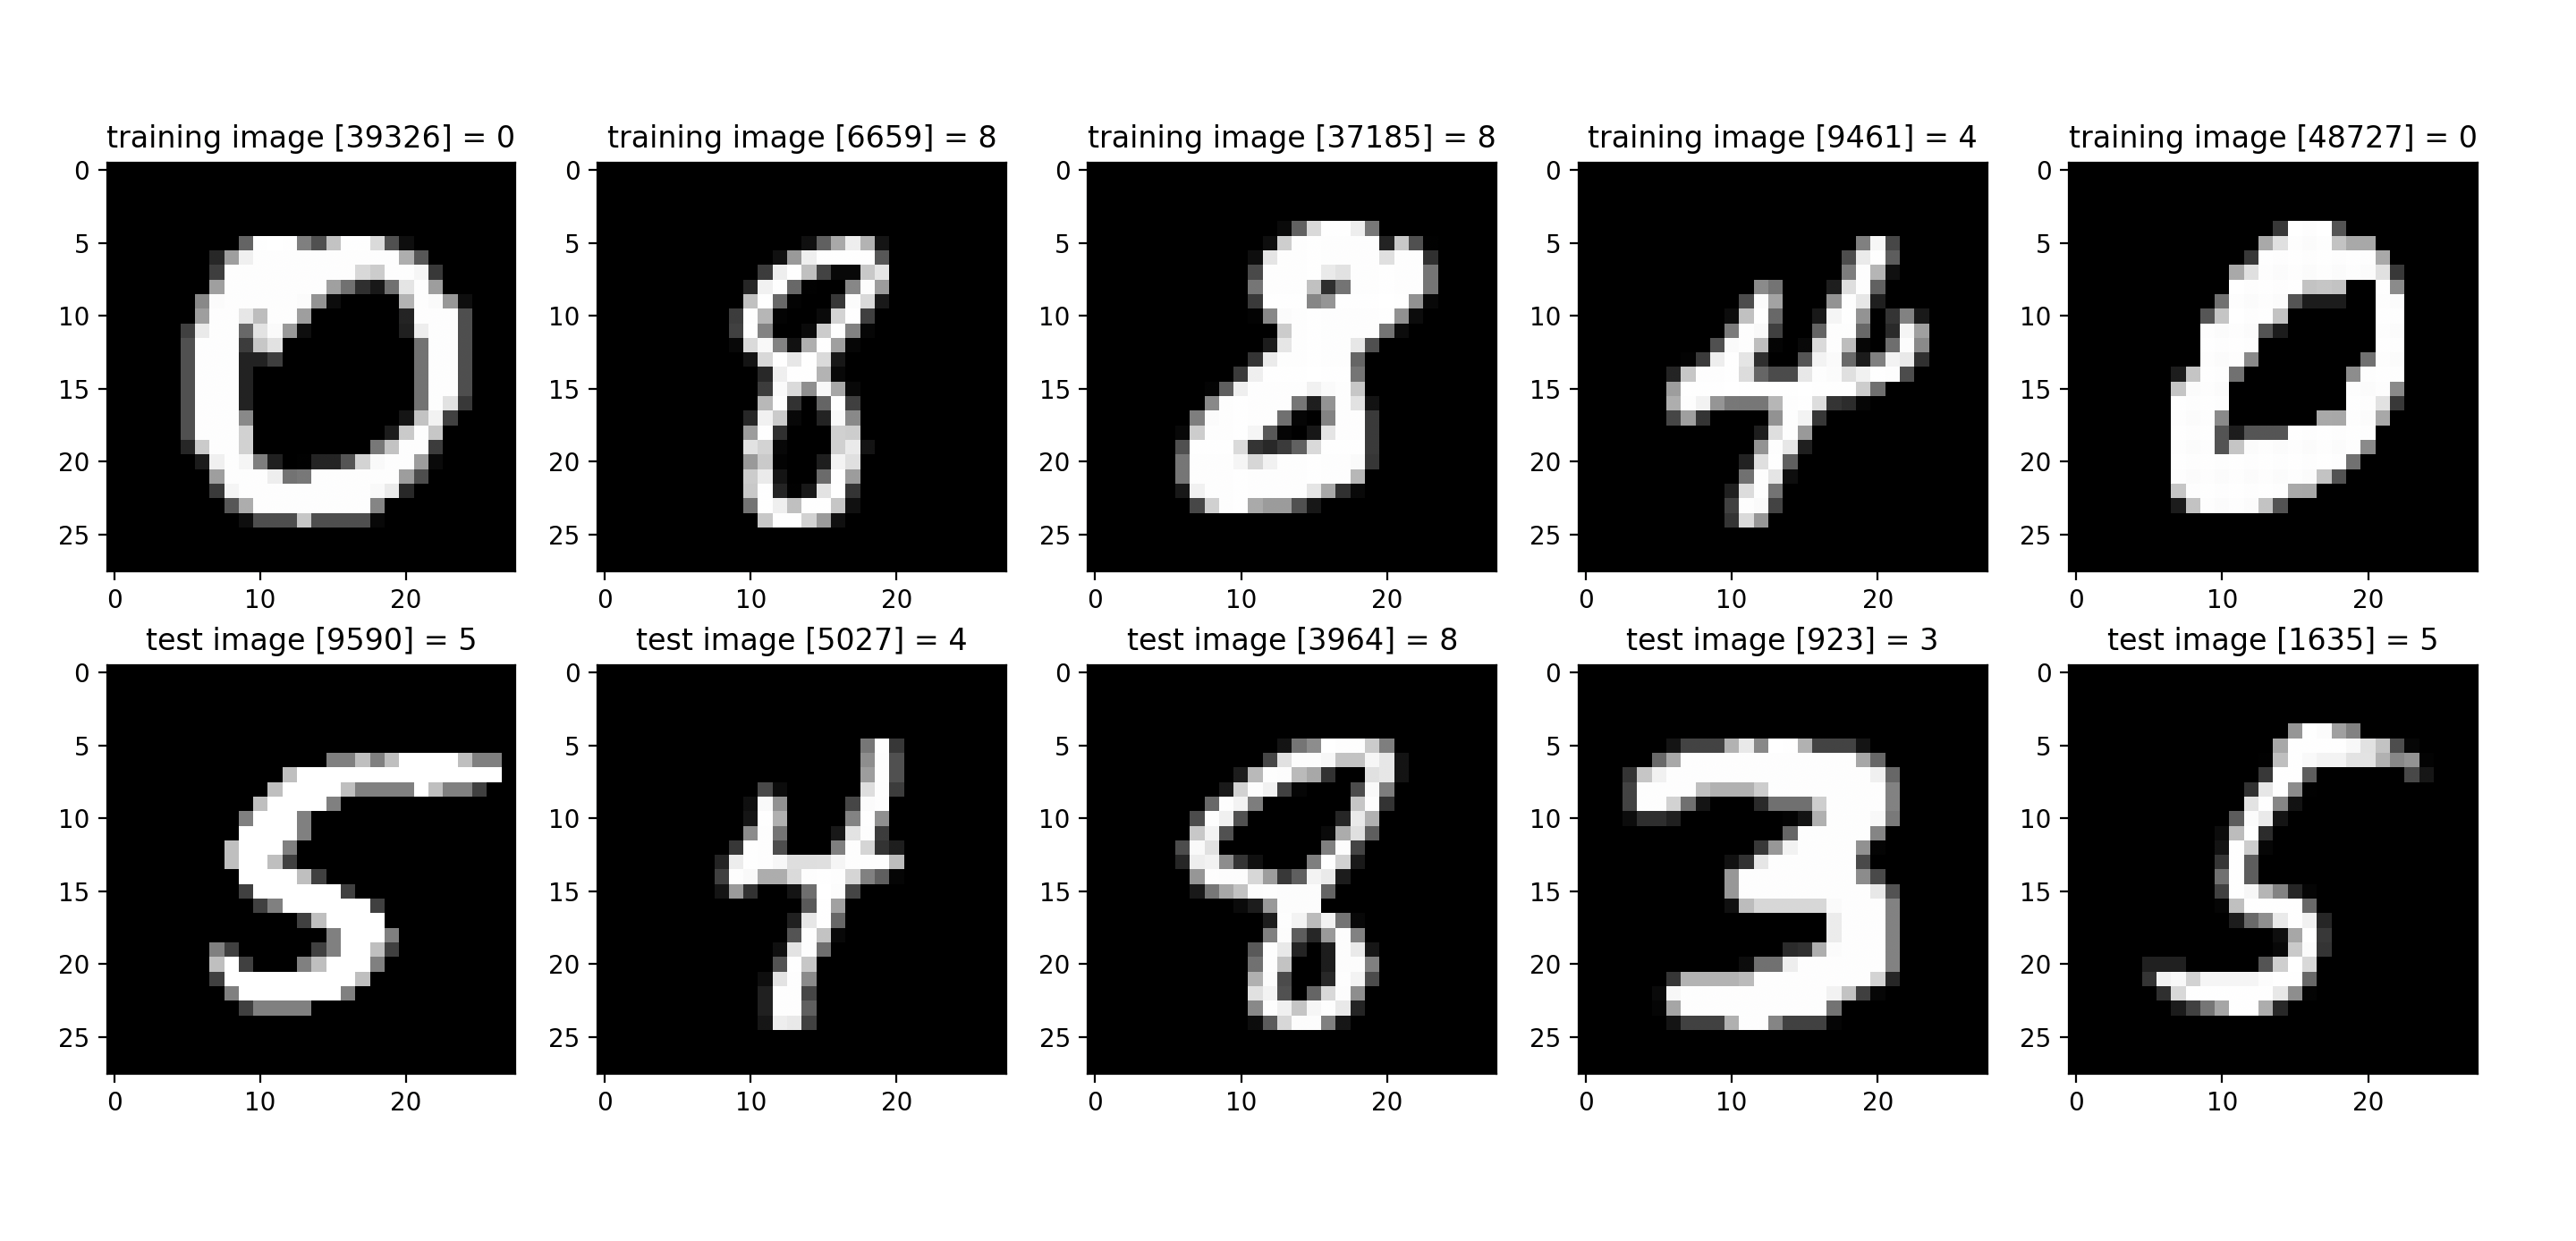
\includegraphics[width=\linewidth]{images/sample_images.png}
  \caption{Samples images and their labels}
\end{figure}

\section{Code}

I have used the data loader to load the train and test samples with their labels and I have written a function to display 5 random training samples and 5 random testing samples.

\lstinputlisting[language=Python, caption=loader.py]{../src/loader.py}
\lstinputlisting[language=Python, caption=main.py]{../src/main.py}

\section{Next Steps}

Since I am able to load and explore the data, I am planning to get started on GAN next. I am currently going through the GAN paper and trying to see if I can figure out implementation details from that paper. If I get stuck on GAN, I'll start implementing VAE in parallel.
\end{document}
